\documentclass[tikz,border=5pt]{standalone}
\usepackage{tikz}
\begin{document}
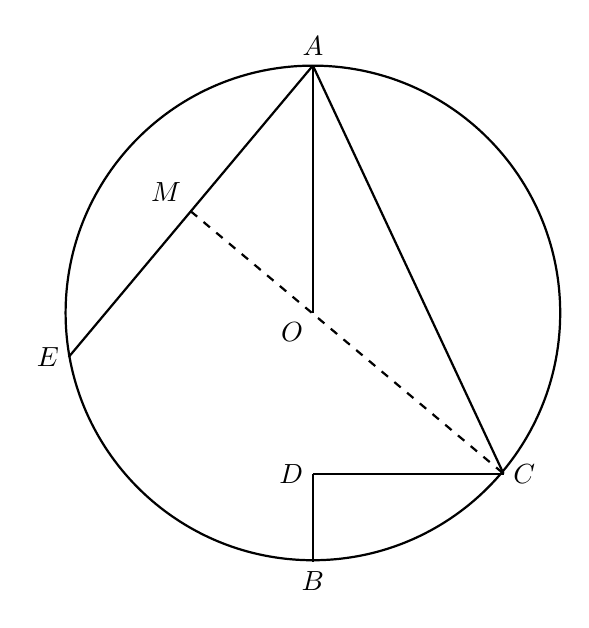
\begin{tikzpicture}[scale=0.02]
  % 坐标以像素为单位，原点为圆心 O，y 轴向上
  \coordinate (O) at (0,0);
  \coordinate (A) at (0,157);
  \coordinate (B) at (0,-158);
  \coordinate (D) at (0,-102);
  \coordinate (C) at (121,-102);
  \coordinate (E) at (-155,-28);
  \coordinate (M) at (-77.5,64.5);

  % 圆
  \draw[line width=0.8pt] (O) circle (157);

  % 线段 AE、AC、DC
  \draw[line width=0.8pt] (A) -- (E);
  \draw[line width=0.8pt] (A) -- (C);
  \draw[line width=0.8pt] (D) -- (C);

  % 竖直线 AB 去掉线段 DO 的笔画，只保留 A–O 与 D–B
  \draw[line width=0.8pt] (A) -- (O);
  \draw[line width=0.8pt] (D) -- (B);

  % 虚线 MC（经过 O）
  \draw[dashed, line width=0.8pt] (M) -- (C);

  % 点 O 的标记
  \fill (O) circle (2pt);

  % 标签
  \node[above] at (A) {$A$};
  \node[below] at (B) {$B$};
  \node[right] at (C) {$C$};
  \node[left]  at (D) {$D$};
  \node[left]  at (E) {$E$};
  \node[above left] at (M) {$M$};
  \node[below left] at (O) {$O$};
\end{tikzpicture}
\end{document}
